\section{Method}

\subsection{Singularity}
The Singularity container were build using a so called "receipt", which tells Singularity how to create the image and what to install inside it. The recipe was added to Singularity Hub, a library were Singularity containers can be uploaded, built and shared \cite{singularity-hub}.

To complete the workflow from raw data to protein quantification results, several other software had to be included in the container, which are listed below.

\subsubsection{MSconvert}
There are a multitude of different types of MS data types, each of which has different file formats. However, only one specific file format is compatible with Quandenser, namely files of type mzML, a general MS data format \cite{mzml-format}. To combat the problem with incompatible data, a software named \textit{Msconvert} was added to the workflow, which can convert MS data from a multitude of vendor formats to the general MS data format needed to run Quandenser \cite{proteowizard}. Due to conversion from vendor formats with Msconvert only works on Windows operative systems, another solution was needed, since the Singularity image was based on Ubuntu, a Linux operative system. The solution was to another type of software called \textit{Wine}, which adds an compatibility layer in POSIX systems (which includes Linux), to run Windows software in a POSIX environment \cite{wine}. The Singularity image was based on another image created by the proteowizard developers, which includes all the necessary components to run Wine and MSconvert \cite{docker-image} \cite{docker-howto}.

\subsubsection{Crux}
Crux is an open source mass spectrometry analysis toolkit available for Linux, Windows and MacOS \cite{crux}. The purpose of integrating Crux into the image was to use three specific tools; tide-index, tide-search and percolator. Tide-index is a pre-search tool that adds indexes and decoys to the protein data base, which is used by the search tool tide-search, that parses fragmentation spectra and creates peptide-to-spectrum matches (PSMs) \cite{tide-search}. Percolator is a post-search tool, that separates peptide targets from decoy PSMs \cite{percolator}. In combination, the tools were used to post-process the output from Quandenser to prepare it for the software triqler, explained in the next section.

\subsubsection{Triqler}
Triqler is an software which uses using graphical models and Bayesian statistics to find differentially expressed proteins between samples. An important note is that Triqler utilizes both MS2 and MS1 spectra, which improves the overall quantification of proteins \cite{triqler}.

ADD MORE STUFF HERE

\subsection{Nextflow}

\begin{wrapfigure}{r}{5cm}
  \centering
  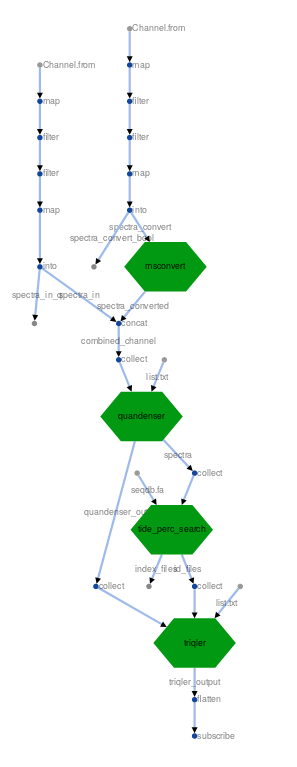
\includegraphics[width=5cm, height=6cm]{pictures/workflow.png}
  \caption{Workflow of the pipeline}
  \label{fig:workflow}
\end{wrapfigure}

Nextflow has integrated compatibility with running software inside Singularity images, which is used to call on the programs contained in the Singularity image. The pipeline is shown in figure \ref{fig:workflow}. Due to Nextflow's capability of running multiple software in parallel, a modified version of Quandenser was added to fully utilize the parallelization. When running the parallelized version of Quandenser in the pipeline, the process is divided into five parts, two of which are parallelizable. The aim was to speed up the calculation time when running large cohorts, since the time scaling of an increased number of files was not a linear relationship to the processing time.

Nextflow also has the benefit of being able to submit processes to workload managers, which are used on HPC clusters to allocate processing time for users. To be able to run the pipeline on HPC clusters, the pipeline is outfitted with an profile to submit processes via SLURM, the current workload manager on UPPMAX, to allow users of the pipeline to run the pipeline on clusters.

To

\subsection{Quandenser-pipeline GUI}
To integrate the Singularity image and the Nextflow pipeline, a GUI was created and packed into the image. Pyside2 was used to create the GUI, which is an open source GUI framework based by the Qt framework \cite{pyside2}. A shell script handling installing Singularity, downloading the image from Singularity Hub and starting the GUI was created to allow users to easily use the pipeline. Figure \ref{fig:GUI_workflow} shows the GUI workflow.

\begin{figure}[!htbp]
  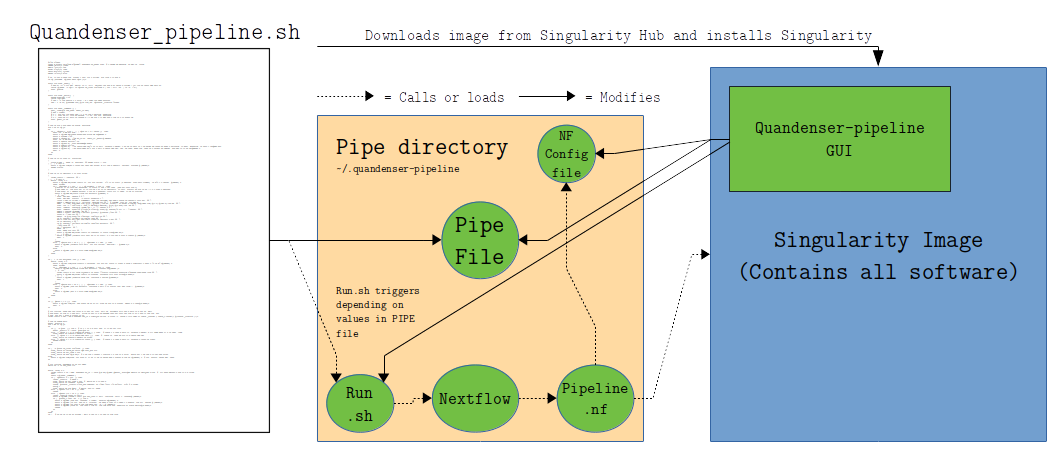
\includegraphics[width=\linewidth]{pictures/GUI_workflow.png}
  \caption{GUI workflow of Quandenser-pipeline}
  \label{fig:GUI_workflow}
\end{figure}

\subsection{Analysing bacterial proteomes}
Comparison between established methods, which uses similar workflow management systems were also compared to the created workflow pipeline. Another workflow manager \textit{KNIME} in combination with \textit{OpenMS} was used to compare
After Quandenser has
